\documentclass[conference]{IEEEtran}
\IEEEoverridecommandlockouts
% The preceding line is only needed to identify funding in the first footnote. If that is unneeded, please comment it out.
\usepackage{cite}
\usepackage{amsmath,amssymb,amsfonts}
\usepackage{algorithmic}
\usepackage{graphicx}
\usepackage{textcomp}
\usepackage{fancyhdr} 
\usepackage{lipsum}
\usepackage{acronym}
\usepackage{xcolor}
\usepackage{hyperref}
\usepackage{caption}
\usepackage{subcaption}
\usepackage{booktabs}
\usepackage{multirow}
\usepackage{float}


\def\BibTeX{{\rm B\kern-.05em{\sc i\kern-.025em b}\kern-.08em
    T\kern-.1667em\lower.7ex\hbox{E}\kern-.125emX}}

% Set up the header and footer
\pagestyle{fancy}
\fancyhf{} 
\fancyhead[R]{Foundations of Machine Learning} 
\fancyfoot[C]{\thepage} 

\begin{document}

\title{Intel Image Scene Classification of Landscapes\\
{\footnotesize \textsuperscript{}

Image Scene Classification of Multiclass \\ 

DETI - Foundations of Machine Learning \\

University of Aveiro, Portugal \\ 

Teacher: Petia Georgieva \\

}
}

\author{\IEEEauthorblockN{1\textsuperscript{st} João Afonso Ferreira}
\IEEEauthorblockA{\textit{MIECT} \\
ferreiraafonsojoao@ua.pt
}
\and
\IEEEauthorblockN{2\textsuperscript{nd} Rafael Curado}
\IEEEauthorblockA{\textit{MECT} \\
rafael.curado@ua.pt
}
}

\maketitle

\begin{abstract}
 This document describes an approach to the Intel Image Scene Classification of Landscapes, a multi-class classification issue with six classes: buildings, forests, glaciers, mountains, seas, and streets. The dataset, obtained via Kaggle, has a wide collection of photos representing various classifications. The primary goal is to create a strong **ResNet50** model that can accurately classify photos into their respective categories. In addition to the ResNet50 model, this study evaluates the performance of various machine learning models on this dataset, including **Random Forest (RF)** and **K-Nearest Neighbours (KNN)**, to determine the best model for this classification job. Furthermore, the study compares the collected results to cutting-edge approaches and related studies to provide a complete evaluation of the proposed strategy. This approach demonstrates the efficacy of deep learning approaches, specifically ResNet50, for picture classification challenges while also laying the groundwork for future computer vision research and development.
\end{abstract}

\vspace{1em}

\begin{IEEEkeywords}
Supervised Machine Learning,
Image Scene Classification,
Landscape Classification,
Random Forest,
K-Nearest Neighbors,
Image Processing,
Deep Learning,
Neural Networks,
Data Augmentation,
Performance Comparison
\end{IEEEkeywords}

\section{Introduction}
Over the past few years, machine learning has made significant advancements in a variety of disciplines, including picture categorization, enabling novel solutions to real-world problems. Among these, landscape picture classification is a crucial topic with several applications in environmental monitoring, urban planning, tourism, and other fields. The capacity to automatically detect and categorize natural landscapes enables machine learning models to tackle tasks like land use analysis, wildlife habitat assessment, and content tagging on digital platforms, opening the way for better decision-making and operational efficiency.

Recent advances in computer vision, particularly the invention of convolutional neural networks (CNNs), have transformed the field of picture classification \cite{kri2017}. Modern architectures such as ResNet, VGG, and EfficientNet offer excellent tools for tackling the complexities of this categorization issue. The purpose of using these methods is to create a strong system capable of discriminating visually comparable categories, such as mountains and glaciers or streets and buildings. This not only highlights modern algorithms' capabilities, but also emphasizes their flexibility to different and demanding datasets. A successful deployment of such a system has positive consequences, such as automating landscape analysis, assisting with environmental conservation efforts, and improving digital content management.

Furthermore, this research looks into the optimization of machine learning models for real-world applications. This includes normalizations and standardizations, optimization of hyperparameters, using data augmentation approaches, and resolving potential limits including overfitting and class imbalance. 

This research aims to demonstrate the usefulness of modern machine learning approaches and make a comparison between them in terms of performance. Therefore, it starts with the State of the Art Review that examines contemporary approaches and new developments in image classification. The varied Kaggle-sourced dataset used for training and assessment is described in the Dataset Overview.

The data pretreatment procedures, such as dataset splitting, image resizing, normalization, class encoding, data augmentation, and K-Fold Cross Validation, are described in the Methods section. In order to evaluate the effect of network depth, it next looks at Convolutional Neural Networks (CNNs), conducting a layer architecture model experience, testing models that have one to five convolutional layers.

The Evaluation and Result Comparison sections that follow evaluate and contrast the performance of various models. In order to compare with deep learning techniques, the project also incorporates conventional machine learning techniques like Random Forest and K-Nearest Neighbours. ResNet50 has a special section on model customization, training, and evaluation.

\section{State of the art review}
In recent years, various studies have looked into the use of machine learning and computer vision algorithms for landscape image classification. This review focuses on key contributions that directly address the classification of natural scenes into various groups, while also providing insights into approaches and their usefulness. The Intel Image Classification Dataset is a valuable resource for scene classification tasks, and it is frequently utilized in research on deep learning approaches for landscape classification. The following study from Luo et al. and GitHub repository specifically used the Intel Image Classification Dataset, the same one used for this project, exploring various models and techniques for improving landscape scene classification performance. The other research studies cited in this section are on global picture classification tasks, which, while significant to the larger topic, do not use the same dataset.

Luo et al. 's study used several machine learning models, such as Random Forest (RF), Support Vector Machines (SVM), Artificial Neural Networks (ANN), and Convolutional Neural Networks (CNNs) \cite{luo2019}. The dataset's category structure and scale make it an excellent benchmark for comparing model performance, demonstrating CNNs' supremacy due to their capacity to learn hierarchical spatial features. The scientists next studied how fine-tuning CNN layer components and changing parameters improved classification accuracy, resulting in competitive results across multiple landscape categories. This study is very useful for investigating several techniques for solving a multi-class landscape image classification challenge.

 Another application of the Intel Image Classification dataset can be found in this GitHub repository that uses Convolutional Neural Networks (CNNs) and pre-trained models such as ResNet50 \cite{githubpratim}. The ResNet50 model outperformed with a test accuracy of 95.3\%, demonstrating its usefulness in scene classification. This result demonstrates the model's capacity to capture complex elements inside natural landscapes, making it a great choice for multi-class scene classification problems. The implementation in this repository serves as an accessible starting point for academics seeking to apply similar techniques to the Intel Image Classification dataset.

Zeng et al.'s \cite{zeng} work "Deep Learning for Scene Classification: A Survey" provides a comprehensive overview of key advances in scene classification, a fundamental and demanding subject in computer vision. The review investigates how the use of large-scale datasets and deep learning approaches has resulted in significant advances in scene representation and classification. It examines how deep learning models, specifically Convolutional Neural Networks (CNNs), have evolved to learn powerful feature representations from raw data, revolutionizing scene categorization tasks. It also outlines prospective research prospects, emphasizing areas where future developments can continue to push the limits of scene classification. This survey is an invaluable resource for understanding the current landscape of deep learning in scene categorization, as well as insights into the field's future prospects.

The article "Remote Sensing Image Scene Classification by Transfer Learning to Augment the Accuracy" by S. Thirumaladevi et al. investigates the use of transfer learning to improve scene classification accuracy with remote sensing images \cite{Thirumaladevi}. The authors used pre-trained models like AlexNet and VGG for feature extraction, illustrating how the second fully connected layer of these models can be used to extract features that are then classified using Support Vector Machines (SVM). The paper also looks into changing the pre-trained network's final layers using transfer learning to improve adaptability to new datasets. The application of deep learning and transfer learning in this study provides crucial insights for improving scene classification in remote sensing, and can be extended to comparable landscape scene classification challenges.

Wenmei Li et al.'s paper "Classification of High-Spatial-Resolution Remote Sensing Scenes Method Using Transfer Learning and Deep Convolutional Neural Network" proposes a novel method for classifying high-spatial-resolution remote sensing (HSRRS) images that combines transfer learning and deep convolutional neural networks \cite{Li}. The paper solves the issue of limited high-quality labeled datasets for deep learning model training by adapting pre-trained networks such as VGG19, ResNet50, and InceptionV3 to HSRRS scenarios using transfer learning. These pre-trained ImageNet2015 models have their convolutional layers transferred to a new TL-DeCNN model, which is fine-tuned using a small number of HSRRS examples. The experimental results show that this strategy outperforms direct model training on few-shot examples, producing superior classification results while avoiding overfitting. This strategy demonstrates transfer learning's potential for overcoming the limitations of insufficient data in high-resolution remote sensing picture classification, making it a valuable tool for landscape and scene classification problems.

The related work discussed in this section is comprehensively summarized in Table~\ref{tab:state_of_art}. This table highlights the key studies, the datasets they utilized, the models and techniques they employed, and the results they achieved. By providing a comparative overview, the table underscores the advancements in landscape image classification and illustrates the effectiveness of various machine learning and deep learning approaches in addressing this domain-specific challenge.

\begin{table}[ht]
\centering
\resizebox{0.5\textwidth}{!}{%
    \begin{tabular}{llp{1.5cm}p{2.5cm}p{3cm}p{2cm}}
        \toprule
        \textbf{Author(s)} & \textbf{Year} & \textbf{Dataset} & \textbf{Models/Techniques} & \textbf{Results} & \textbf{Notes} \\
        \midrule
        Luo et al. \cite{luo2019} & 2019 & Intel Image Classification & RF, SVM, ANN, CNNs & CNNs demonstrated superior performance (Testing Error: \textit{14.54\% Vs 40.03\%} (RF)) & Explored fine-tuning CNN layers for improved accuracy \\

        GitHub Rep \cite{githubpratim} & 2020 & Intel Image Classification & CNNs, ResNet50 & Achieved 906 \% (CNN) 95.3\% (ResNet50) test accuracy & Utilizes a 10 convolutional layers CNN model and a pre-trained ResNet50 model \\
        Zeng et al. \cite{zeng} & 2019 & Various & Deep Learning, CNNs & Comprehensive overview of advancements & Focused on large-scale datasets and feature representation \\
        Thiruma. et al. \cite{Thirumaladevi} & 2020 & Remote Sensing Images & Transfer Learning, AlexNet, VGG, SVM & Improved classification accuracy & Applied transfer learning to adapt pre-trained networks \\
        Wenmei Li et al. \cite{Li} & 2020 & High-Spatial-Resolution Remote Sensing & Transfer Learning, VGG19, ResNet50, InceptionV3 & Outperformed direct model training  producing superior classification results while avoiding overfitting & Addressed limited high-quality labeled datasets \\
        \bottomrule
    \end{tabular}
}
\caption{Summary of State-of-the-Art and Related Work in Landscape Image Classification}
\label{tab:state_of_art}
\end{table}


\section{Dataset Overview}
The dataset for this project is a collection of natural scene photographs from around the world donated by Intel for an image classification challenge available at \url{https://datahack.analyticsvidhya.com} and at Kaggle \cite{kaggleDataset}. The collection contains roughly 25,000 photos, each measuring 150x150 pixels and classified into six categories: \textit{Buildings, Forest, Glacier, Mountain, Sea, and Street}, as it is possible to observe in Fig. \ref{fig:visualizationClassesData}. Categories are encoded as follows: Buildings - 0, Forest - 1, Glacier - 2, Mountain - 3, Sea - 4, and Street - 5.

The dataset is separated into three subsets: training, testing, and prediction. The training set has around 14,000 photos, distributed as shown in Fig. \ref{fig:classDis}, the test set has about 3,000 images, and the prediction set has about 7,000 images. This separation enables efficient training, validation, and assessment of machine learning models.

The major goal of this collection is to help developers create powerful neural networks capable of appropriately categorizing these photos. The dataset contains a large and diversified variety of nature scenarios, making it a valuable resource for developing and testing image classification models.

\begin{figure}
    \centering
    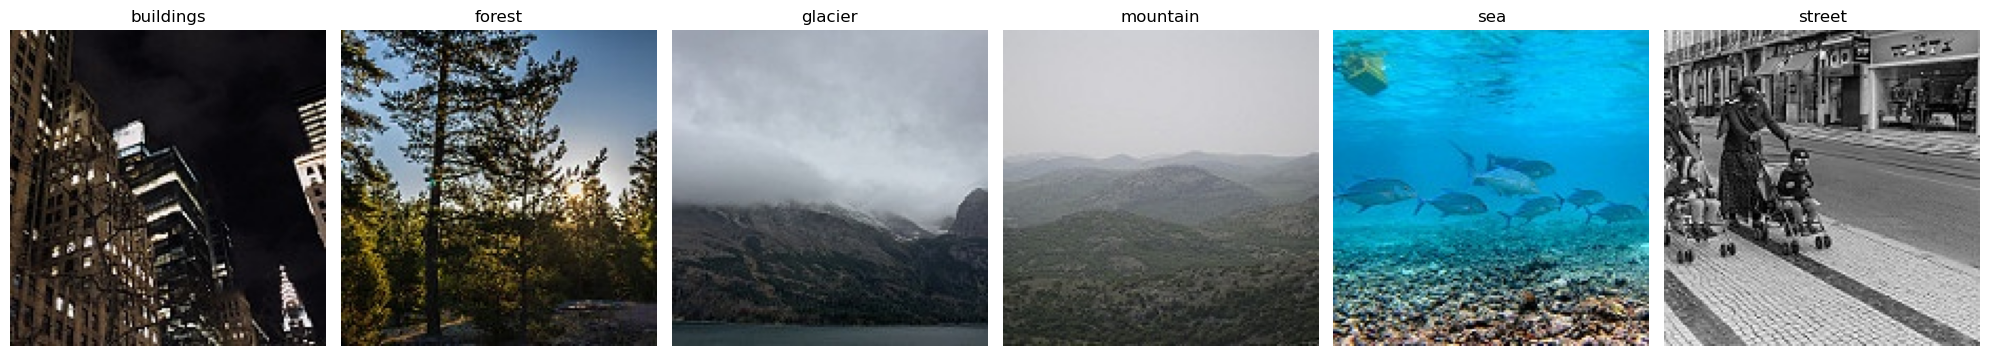
\includegraphics[width=\linewidth]{img/classesVisualisation.png}
    \caption{Visualization of The Six Classes in The Dataset }
    \label{fig:visualizationClassesData}
\end{figure}

\begin{figure}
    \centering
    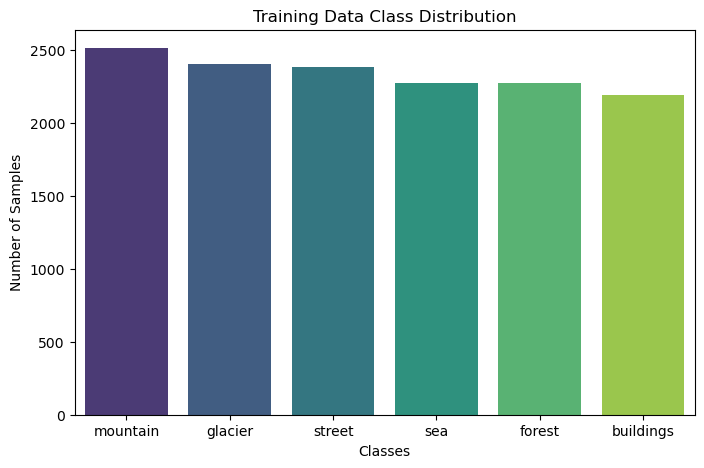
\includegraphics[width=\linewidth]{img/classDistribution.png}
    \caption{Class Distribution}
    \label{fig:classDis}
\end{figure}


\section{Methods}
\label{sec:meth}

\subsection{Data PreProcessing}
Preprocessing the dataset is an important step in preparing it for use in the \ac{CNN} model. The primary purpose is to improve the dataset for optimal model performance by transformations such as data augmentation, standardization, and partitioning it into training, validation, and testing sets.

\subsubsection{Dataset Splitting}
The data was divided into three subsets:
\begin{itemize}
    \item \textbf{Training Set}: This subset, representing 90\% of the data in the training directory, was useed to train the models. This set receives data augmentation, allowing the model to learn from a wide range of image variances.

    \item \textbf{Validation Set}: A subset, Comprising 10\% of the data in the training directory, used to track the model's performance during training and avoid overfitting and also used to tune hyperparameters, ensuring the model performs well on unseen data. 

    \item \textbf{Test Set}: A distinct set used to assess the final model's performance following training. This collection was not augmented, and it represents the model's genuine capacity to generalize to new, previously unknown data.
\end{itemize}

A visualization of the data splitting process is presented in the Fig. \ref{fig:dataSplit}.

\begin{figure} [ht]
    \centering
    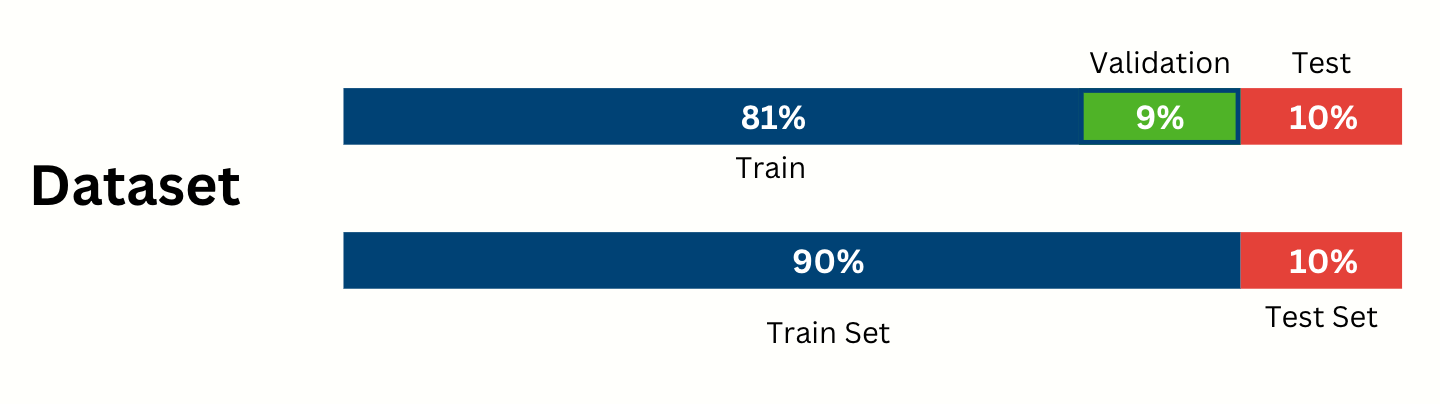
\includegraphics[width=\linewidth]{img/dataSplitting.png}
    \caption{Data splitting process}
    \label{fig:dataSplit}
\end{figure}

\subsubsection{Image Resizing}
All input images were scaled to the same shape of 150x150 pixels. This step is important to achieve uniformity because CNNs require set input sizes for processing. Resizing is essential when working with photos of varied proportions, since this process allows generalization throughout all images.

\subsubsection{Data Normalization}
Normalization was used to guarantee that the data inputs were on a comparable scale so that \ac{ML} models could handle them efficiently \cite{normalization}. Dividing by 255 scaled all pixel values to the range [0, 1]. This procedure converts all pixel values, which originally ranged from 0 to 255, into a consistent scale, allowing for faster convergence during model training. Normalizing the input allows the model to learn patterns more efficiently. This technique was performed using \textit{ImageDataGenerator} from tensorflow \cite{ImageDataGenerator}.

\subsubsection{Class Encoding}
For multi-class classification, the class labels were encoded as integers for each class \cite{encoding}. The \textit{ImageDataGenerator} was set to use sparse class labels, which provide integer values rather than one-shot encoded vectors. This method is efficient and uses less memory. The Keras ImageDataGenerator was used to load, preprocess, and supplement the photos.

For the training set, both augmentation and normalization were used. Only normalization was used on the validation and test sets to ensure that preprocessing was consistent throughout the training and assessment stages.

\subsubsection{Data Augmentation}
Data augmentation approaches were used to reduce overfitting and boost training data diversity. These changes produce updated versions of the images that expose the model to different variances, allowing it to generalize more effectively. The applicable augmentations included \textit{horizontal flips} (images are randomly flipped along the horizontal axis), \textit{shear range} (shears the photos, causing subtle distortions - noise), \textit{zoom range changes} (random zooming in and out to simulate varying distances from the items), \textit{rescaling} (all pixel values were rescaled by a factor of 1/255, bringing the input images into the range of [0, 1]). All these augmentations/techniques help to accelerate training and stabilize the model during its learning process.

By performing these preprocessing steps, the dataset is well prepared for training robust \ac{ML} models, which improves its capacity to generalize and make credible predictions on previously unseen data.

\subsubsection{K-Fold Cross Validation}
As part of the data preprocessing and model validation technique, k-fold cross-validation was used to guarantee a reliable assessment of these models.

In order to do K-fold cross-validation, the dataset is divided into k folds of equal size. One fold for each of the k iterations is called the validation set, while the other (k-1) folds are called the training set. By ensuring that each data point is used for both training and validation, this procedure offers a thorough evaluation of the model's performance across various data subsets.

Fivefold cross-validation was used in this study, which means that the dataset was split into five folds. Every fold was used as the validation set once during the five training and validation cycles for each model. The performance metrics were then averaged across all folds to obtain an overall evaluation of each model's efficacy.

Upon applying k-fold cross-validation, it was observed that only the ResNet50 model exhibited significant performance improvements compared to its performance without cross-validation (Table. \ref{tab:resnet50_results}). When assessed using the k-fold method, the other models—such as CNNs with 1–5 convolutional layers, Random Forest, and KNN—did not demonstrate appreciable improvements.

ResNet50's deep and intricate architecture, effective feature extraction, and the thorough training process made possible by k-fold cross-validation are all responsible for this increase. Conversely, less complex models like Random Forest, CNNs with fewer convolutional layers, and KNN did not show appreciable performance improvements, underscoring the advantages of cross-validation methods for particular models.



\subsection{Convolutional Neural Networks}
For the working dataset, image based one, it was used Convolution Neural Networks, also known as a \ac{CNN}, which is an artificial neural network that has so far been most popularly used for analyzing images for computer vision tasks \cite{deeplizard}.

It is possible to imagine \ac{CNN} as a sort of an artificial neural network that specializes in identifying or detecting patterns. CNNs are excellent for image analysis because of their ability to discover patterns due to their hidden layers called convolutional layers, and these layers are what make a \ac{CNN}. With each convolutional layer, there is this need to specify the number of filters the layer should have, since these filters are actually what detect the patterns.

A CNN typically includes the following key components:

\begin{itemize}
    \item \textbf{Convolutional Layers}: These layers apply convolutional filters to the input image, extracting low-level features (e.g., edges) in the first layers and more complicated features (e.g., forms and textures) in subsequent layers. Convolution is the process of sliding a filter over an image, conducting element-wise multiplication, and summing the results to get a feature map.

    \item \textbf{Activation Function}: Following the convolution procedure, an activation function, often the ReLU (Rectified Linear Unit - Fig. \ref{fig:relu}), is used to induce nonlinearity and assist the model in learning complex patterns.

    \item \textbf{Pooling Layers}: These layers minimize the spatial dimensions of feature maps, lowering computing cost and preventing overfitting. Max-pooling is a typical method for picking the maximum value from a bunch of pixels in a specific region.

    \item \textbf{Fully Connected Layers}: After the convolutional and pooling layers, the feature maps are flattened into a one-dimensional vector and processed through fully connected layers. These layers execute the final categorization using the features learned from the image.
\end{itemize}

The final output layer utilizes a softmax activation function \cite{softmaxactivation} (expressed in eq. \ref{Softmaxfunction_for_multi_class_classification}) to assign the input image to one of the predetermined categories.

\begin{equation}
    P(y_i | \mathbf{x}) = \frac{e^{z_i}}{\sum_{j=1}^{K} e^{z_j}}
    \label{Softmaxfunction_for_multi_class_classification}
\end{equation}
Where \( z_i = w_i^T x + b_i \) represents the \textit{logit} (function no. \ref{logit}, where \( p \) is the probability of the event occurring) for class \( i \) , and the denominator is the sum of the exponentials of all class logits. This ensures that each class has a corresponding probability, and the class with the highest probability is selected for model prediction.

\begin{equation}
    \text{Logit}(p) = \log \left( \frac{p}{1 - p} \right)
    \label{logit}
\end{equation}

\begin{figure}
    \centering
    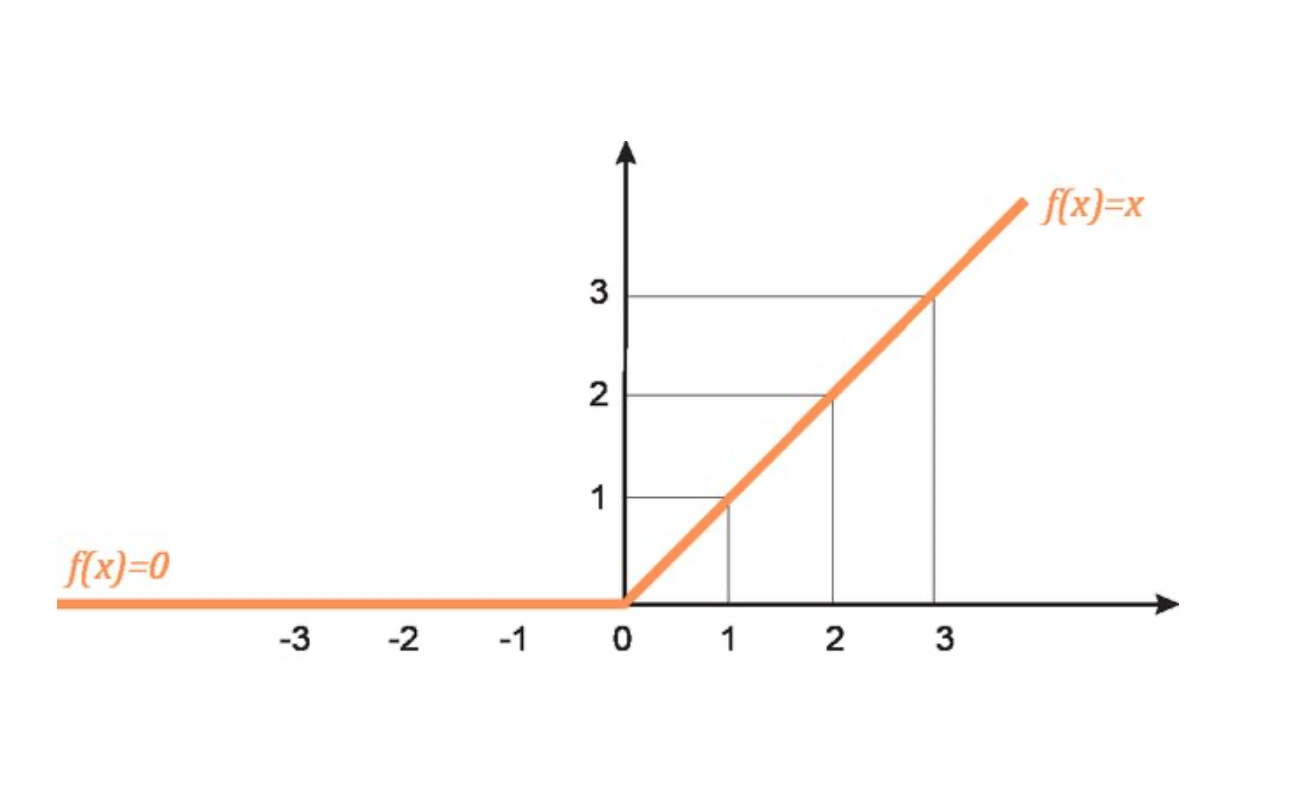
\includegraphics[width=\linewidth]{img/relu.png}
    \caption{Graphic representation of the ReLU activation function (image taken from \cite{relumax})}
    \label{fig:relu}
\end{figure}


\subsubsection{Experiment Process for CNN Models with 1 to 5 Convolutional Layers} 
Each CNN model had a similar architecture but varying depths, which were defined by the number of convolutional layers:
\begin{enumerate}
    \item The \textbf{input layer} received photos with dimensions of 150x150x3, representing RGB images.

    \item \textbf{Convolutional Layers}: For each model, the number of convolutional layers ranged from 1 to 5. Each convolutional layer employed filters of size (3x3) and the ReLU activation function. The number of filters in each layer increased gradually with each successive layer, beginning with 32 filters in the first layer and increasing by 32 filters for each succeeding layer.

    \item \textbf{Batch normalization} was used after each convolutional layer to help stabilize the learning process and increase convergence.

    \item \textbf{Max-Pooling}: After each convolutional layer, a 2x2 max-pooling layer was added to minimize the spatial dimensions of the feature maps and prevent overfitting.
    
    \item \textbf{Fully Connected Layers}: After the convolutional and pooling layers, the output was flattened into a 1D vector, which was then followed by a dense layer with 128 units and a 0.5 dropout rate to reduce overfitting.

    \item The \textbf{output layer} had units equal to the number of classes in the dataset (6 in this case), and it utilized the softmax activation function to generate probabilities for each one.

\end{enumerate}

Each model was built using the Adam optimizer \cite{adam}, an efficient form of gradient descent. The loss function employed was categorical crossentropy, which is suitable for multi-class classification issues, and the evaluation metric was accuracy \cite{crossentropy}.

For each configuration (1 to 5 convolutional layers), for the \textit{Training Set}, the model was trained using augmented training data (horizontal flips, shearing, and zooming), as previously described. For \textit{Validation Set}, the model's performance was evaluated on a distinct subset of data to prevent \textit{overfitting}.
\textit{Early stopping} was utilized to limit training when the validation loss stopped improving after a given number of epochs (patience = 5). This avoided continuous unnecessary training and decreased the possibility of overfitting \cite{earlyStopping}.
Each model was trained for a maximum of 50 epochs; however, early stopping allowed the training process to be terminated if the model's performance stopped improving.

\subsubsection{Evaluation}
Following training, the models were tested on a separate test set that had not been utilized in training. The evaluation metrics included the following:
\begin{itemize}
    \item \textbf{Test Loss}: The loss value calculated using the test set. 
    
    \item \textbf{Test accuracy} refers to the model's performance on the test set.

    \item A complete \textbf{classification report} was generated, which included precision, recall, and F1-scores for each class.

    \item \textbf{Matthews Correlation Coefficient (MCC)}: A metric that measures categorization performance in a balanced manner by accounting for true positives, true negatives, false positives, and false negatives.
\end{itemize}


\subsubsection{Result Comparison}
The results of models with 1 to 5 convolutional layers were compared to see which architecture performed best in terms of test accuracy, loss, and other evaluation criteria. Additionally, a confusion matrix was created for each model to visualize its performance on each class, including the number of true positives, false positives, true negatives, and false negatives \cite{confmatrix}. These comparisons allowed us to evaluate how increasing the number of convolutional layers affected model performance and generalization.

Table \ref{tab:model_performance} shows performance metrics and results for classification models with different numbers of convolutional layers. After training each model, the classification report from the Scikit-learn library \cite{classreport} was used to calculate precise metrics such as precision, recall, F1-score, and support for each class. The macro-averaged values for precision, recall, and F1-score were calculated to provide a balanced assessment of model performance across all classes, independent of class imbalance. Furthermore, the \ac{MCC}) was calculated as a reliable indicator of the model's overall predictive quality. The accuracy and other metrics were calculated on a test set of 3,000 samples to ensure consistency and comparability between models.

As it is possible to observe from the results presented in the following matrices (Figs. \ref{fig:sub1} - \ref{fig:sub5}) and on the Table \ref{tab:model_performance}, the model with three convolutional layers performs the best in categorizing the six image landscape types. In contrast, the worst performance is seen in a model with three convolutional layers, as evidenced by the absence of the noticeable and typical diagonal in the confusion matrix and from the lower results of the performance metrics.

\begin{table}[ht]
    \centering  
    \begin{tabular}{|c|c|c|c|c|c|}
    \hline
    \textbf{Layers} & \textbf{Accuracy} & \textbf{Precision} & \textbf{Recall} & \textbf{F1-Score} & \textbf{MCC} \\ \hline
    1               & 0.73            & 0.73                        & 0.73                     & 0.72                        & 0.67       \\ \hline
    2               & 0.65            & 0.65                        & 0.65                     & 0.61                      & 0.59       \\ \hline
    \textbf{3}               & \textbf{0.82}            & \textbf{0.83}                        & \textbf{0.83}                    & \textbf{0.83}                        & \textbf{0.80}       \\ \hline
    4               & 0.81            & 0.82                        & 0.82                     & 0.81                        & 0.78       \\ \hline
    5               & 0.82            & 0.83                        & 0.82                     & 0.82                        & 0.78       \\ \hline
    \end{tabular}
    \caption{Performance metrics for models with different numbers of convolutional layers.}
    \label{tab:model_performance}
\end{table}

\begin{figure}[ht]
    \centering
    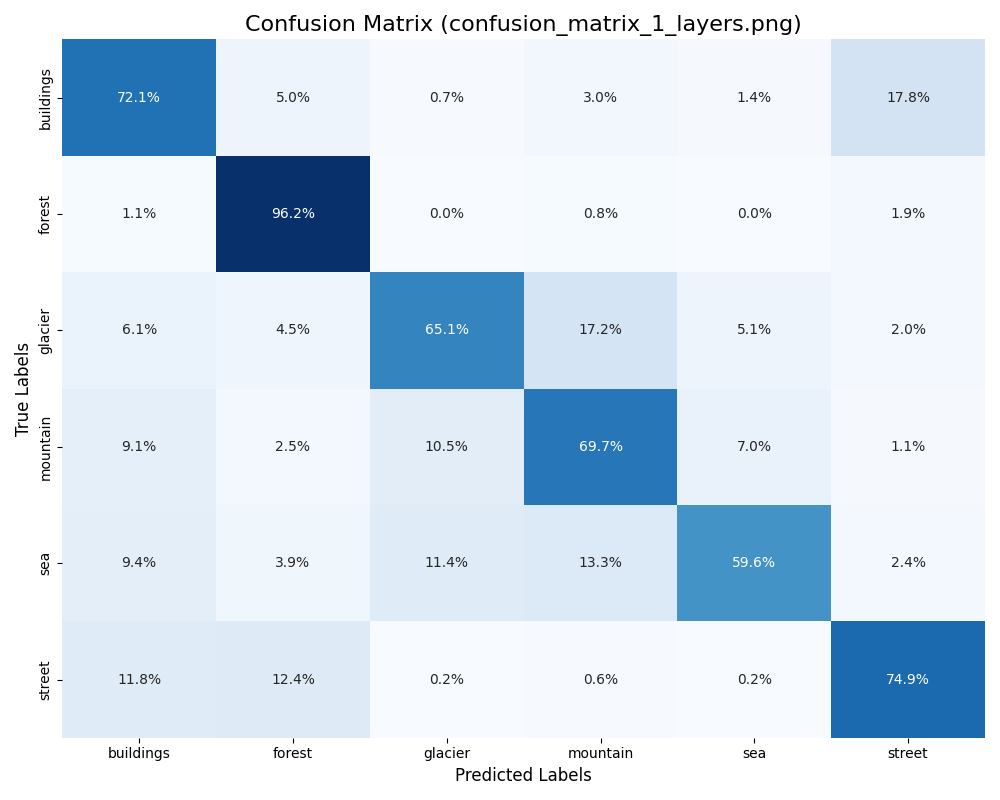
\includegraphics[width=\linewidth]{img/confusion_matrix_1_layers.png}
    \caption{1 Convolutional Layer CNN}
    \label{fig:sub1}
\end{figure}

\begin{figure}[ht]
    \centering
    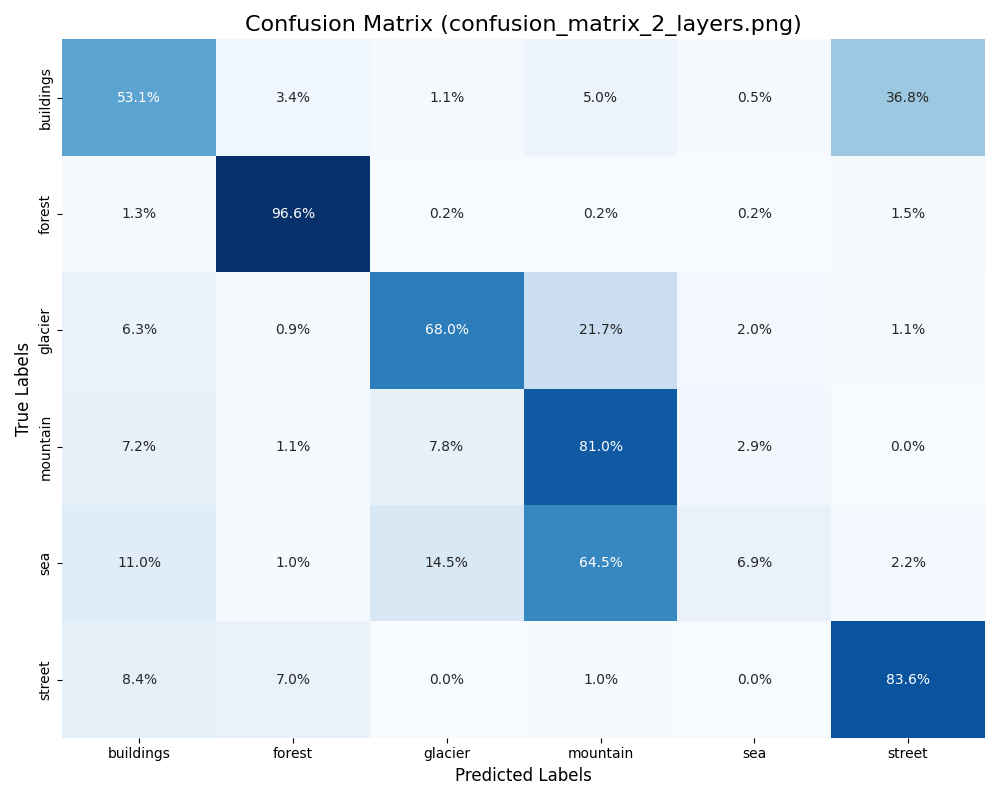
\includegraphics[width=\linewidth]{img/confusion_matrix_2_layers.png}
    \caption{2 Convolutional Layer CNN}
    \label{fig:sub2}
\end{figure}

\begin{figure}[ht]
    \centering
    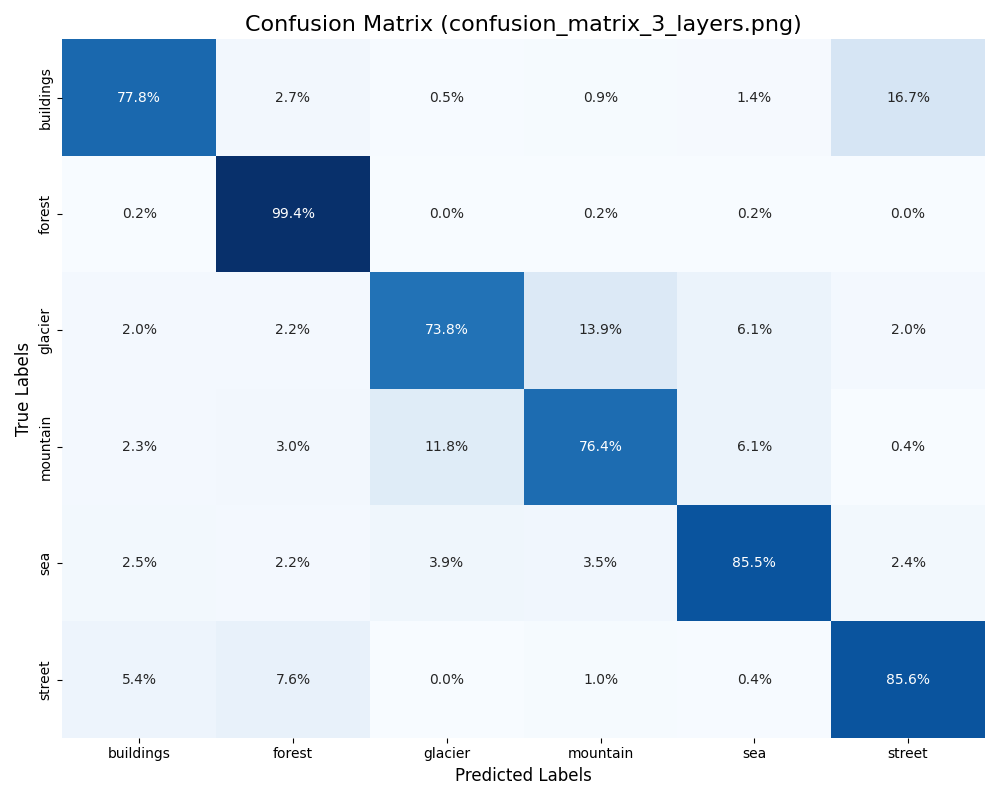
\includegraphics[width=\linewidth]{img/confusion_matrix_3_layers.png}
    \caption{3 Convolutional Layer CNN}
    \label{fig:sub3}
\end{figure}

\begin{figure}[ht]
    \centering
    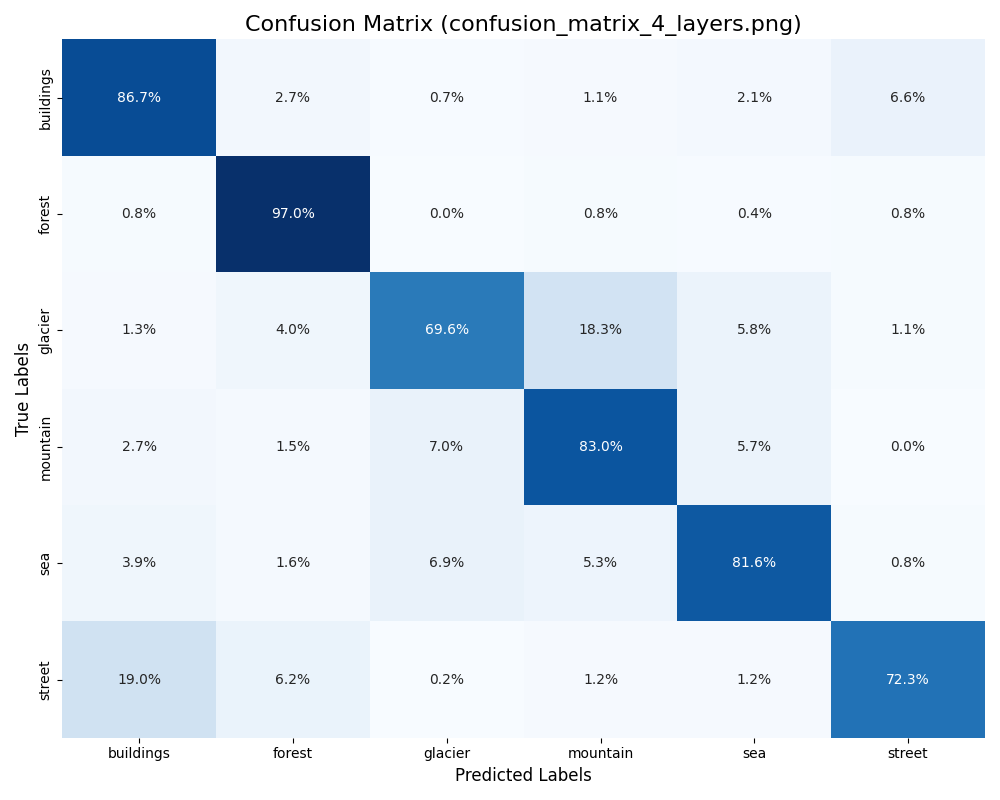
\includegraphics[width=\linewidth]{img/confusion_matrix_4_layers.png}
    \caption{4 Convolutional Layer CNN}
    \label{fig:sub4}
\end{figure}

\begin{figure}[ht]
    \centering
    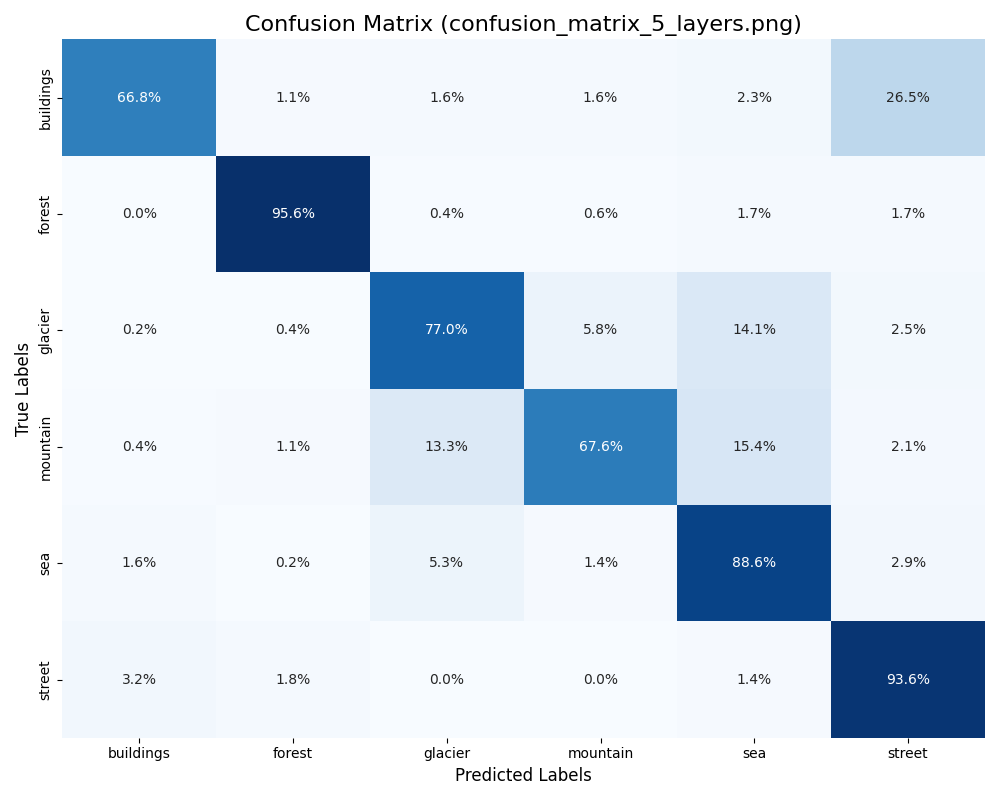
\includegraphics[width=\linewidth]{img/confusion_matrix_5_layers.png}
    \caption{5 Convolutional Layer CNN}
    \label{fig:sub5}
\end{figure}


After identifying the best \ac{CNN} model, it was also plotted a plot of accuracy over epochs (Fig. \ref{fig:accuracycnn}) and \textit{Log loss} over epochs (Fig. \ref{fig:losscnn}),  also known as cross-entropy loss multinomial log loss, is a popular performance metric for assessing classification models with many classes \cite{loglosss}. It assesses the difference between anticipated probabilities and actual class labels. Lower log-loss indicates improved model performance \cite{logloss}. The cost function, as mentioned by Géron et al. \cite{b3} over the whole training set is simply the average cost over all training instances, can be written in a single expression called the log loss, shown in eq. \ref{eq:logloss}. 

\begin{equation}
    J(\theta) = -\frac{1}{m} \sum_{i=1}^m \sum_{c=1}^C y^{(i)}_c \log\left(\hat{p}^{(i)}_c\right)
    \label{eq:logloss}
\end{equation}

\begin{figure} [ht]
    \centering
    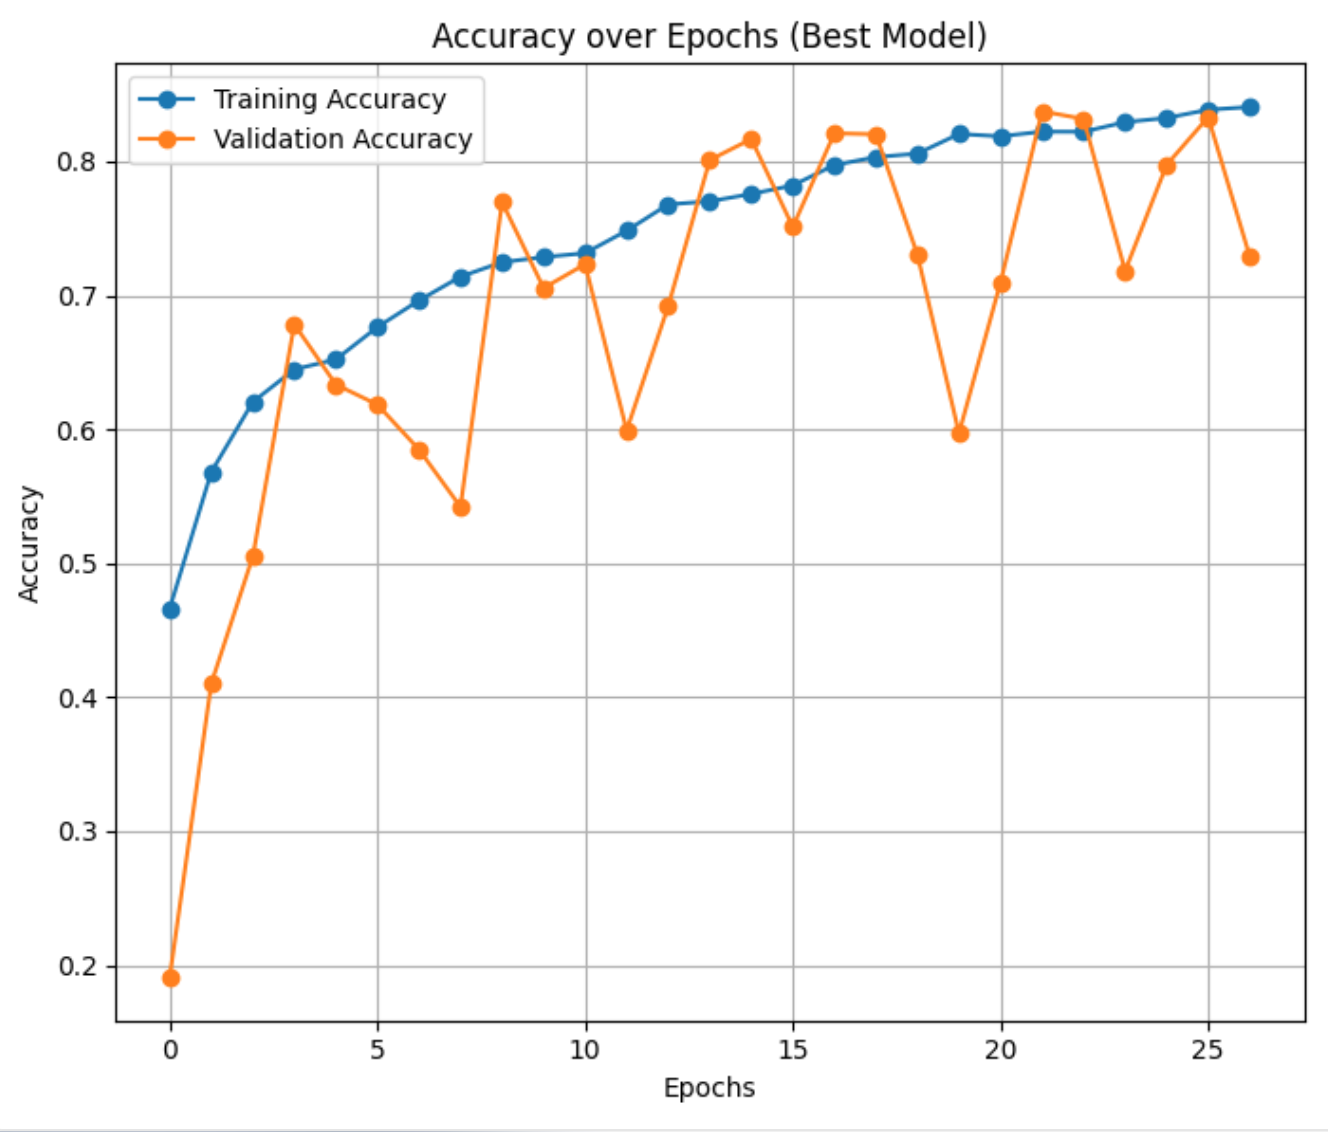
\includegraphics[width=\linewidth]{img/accuracyCNN.png}
    \caption{Accuracy Over Epochs For the Best CNN 3 ConvLayer Model}
    \label{fig:accuracycnn}
\end{figure}

\begin{figure} [ht]
    \centering
    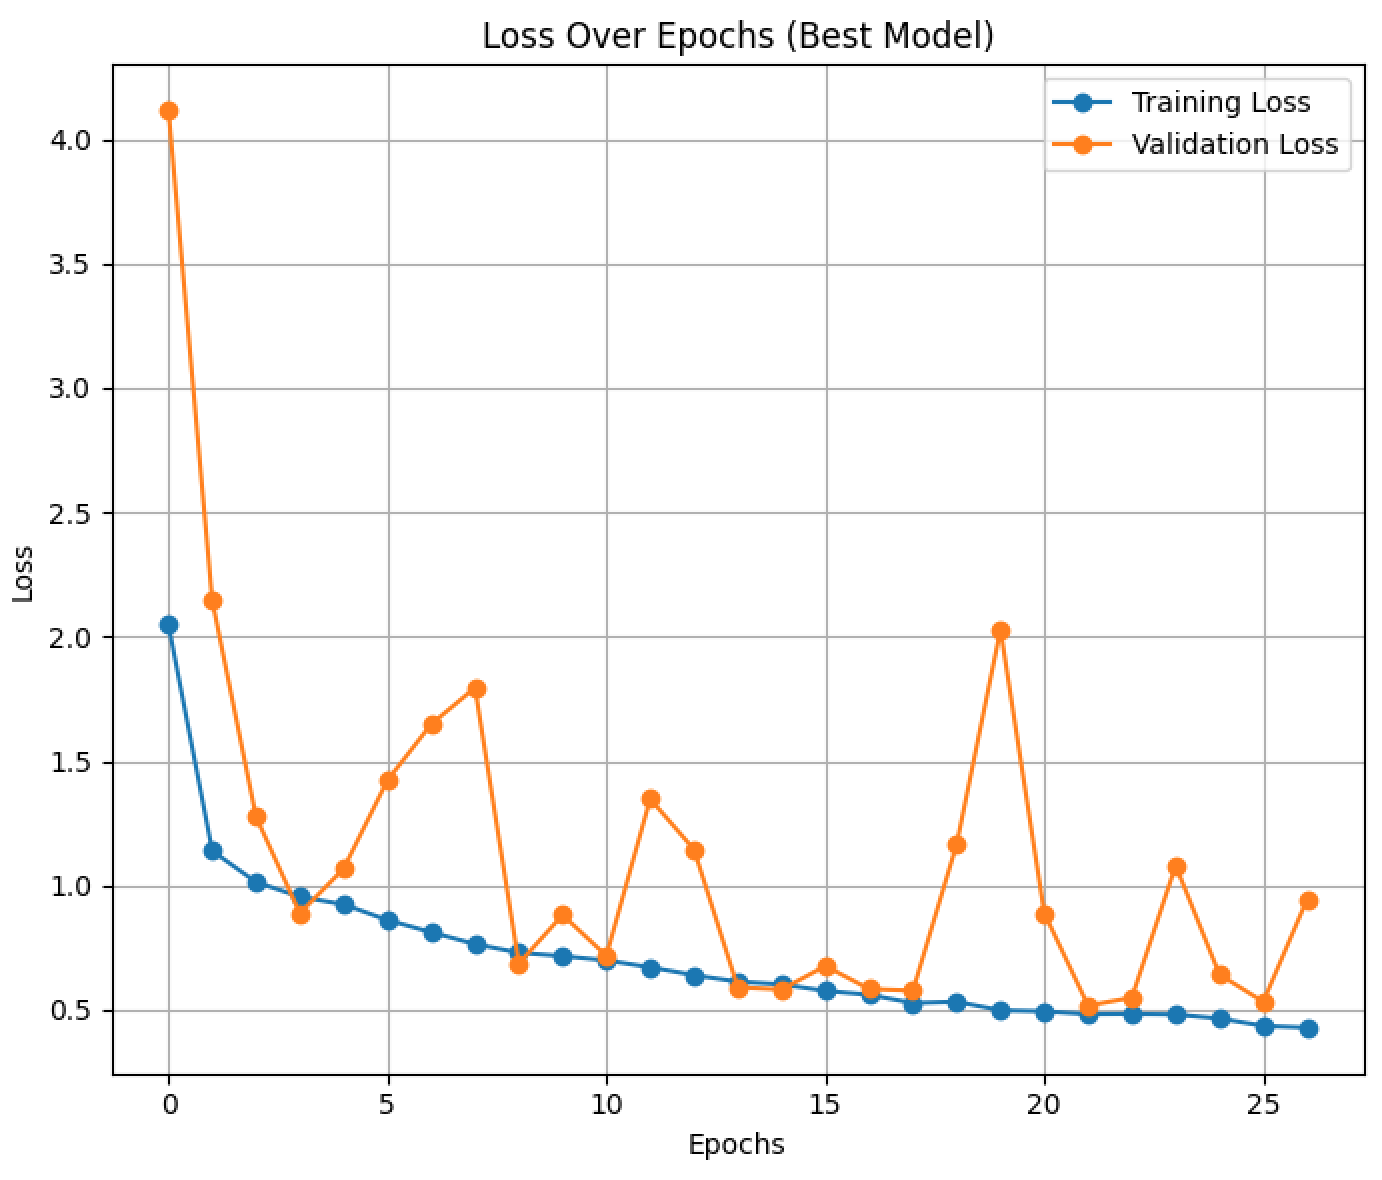
\includegraphics[width=\linewidth]{img/lossCNN.png}
    \caption{Cost/Loss Function Over Epochs  For the Best CNN 3 ConvLayer Model}
    \label{fig:losscnn}
\end{figure}

% MISSING CONFUSION MATRIXES FOR EACH LAYER CNN

 

\subsection{Random Forest and K-Nearest Neighbors}
After assessing the performance of the \ac{CNN}) model, which yielded promising results, it is useful to compare it to other classic machine learning methods. In this section, we show the results of the \ac{RF} and \ac{KNN} models, which were evaluated on the same dataset. The goal is to see if these simpler models can match or beat CNNs in terms of accuracy, precision, recall, and F1 score. The table below highlights the important performance metrics of the Random Forest and KNN models:

\begin{table}[ht]
    \centering  
    \begin{tabular}{|c|c|c|c|c|c|}
    \hline
    \textbf{Models} & \textbf{Accuracy} & \textbf{Precision} & \textbf{Recall} & \textbf{F1-Score} & \textbf{MCC} \\  \hline
    \ac{KNN} & 0.41 & 0.53 & 0.40 & 0.37 & 0.30 \\ \hline
    \ac{RF} & 0.61 & 0.60 & 0.60 & 0.60 & 0.53\\ \hline

    \end{tabular}
    \caption{Performance Comparison of Models: KNN Vs Random Forest}
    \label{tab:comparison_modelsrf}
\end{table}

Observing the Table \ref{tab:comparison_modelsrf}, it is possible to observe that the \ac{KNN} model demonstrates its poor ability to reliably classify image categories, particularly sea and street, which it struggled with the most. While the Random Forest model performed well in some classes, such as forest, it had a poorer overall classification performance than the CNN model, as previously observed.



\subsection{ResNet50}
% RAFA'S PART
The ResNet50 model was another approach that we used to identify photos from the Intel Image Scene Classification. ResNet50, a 50-layer deep convolutional neural network, is a well-known architecture that uses residual connections to alleviate the vanishing gradient problem. This property makes it especially useful for training deep networks and combining transfer learning with pretrained weights. 

ResNet50 consists of multiple convolutional layers, batch normalization, ReLU activations, and residual blocks. The key characteristic is its use of identity and projection shortcuts, which allow the network to "skip" layers, allowing the gradient to flow more effectively during backpropagation. This architecture ensures that the model's performance remains stable as the depth rises.

The key components of ResNet50 are:

\begin{itemize}
    \item \textbf{Convolutional Layers}: gather spatial and hierarchical properties from input images.
    \item  \textbf{Residual Blocks}: Use skip connections to connect a block's input directly to its output, resulting in consistent gradient flow and preventing performance degradation in deeper networks.

    \item \textbf{Bottleneck Design}: Each residual block has a bottleneck structure with three convolutional layers, which reduces computational complexity while preserving feature extraction capability.
    \item \textbf{Global Average Pooling}: replaces completely connected layers, lowering the possibility of overfitting by summarizing feature maps.
\end{itemize}
   
The model was pre-trained using ImageNet \cite{imagenet}, a large-scale image dataset, to take use of features learned from various image categories. During initial training, the pretrained layers were frozen to allow the custom classification head to take priority.


\subsubsection{Model Customization}
For this project, the top layers of ResNet50 were replaced with a customized classification head designed for the six landscape categories. This head includes:

\begin{enumerate}
    \item A GlobalAveragePooling2D layer is used to minimize the spatial dimensions of feature maps generated by the ResNet50 backbone. 
    \item A dense layer with 128 units with ReLU activation that introduces nonlinearity to learn complex dataset-specific patterns.
    \item A 0.5-rate dropout layer that reduces overfitting by randomly deactivating neurons during training.
    \item A final dense layer with softmax activation generating class probabilities for all six categories.
\end{enumerate}

The model was built with the Adam optimizer, which dynamically modifies learning rates, and a sparse categorical cross-entropy loss, which is appropriate for multi-class classification applications.

\subsubsection{Training and Evaluation}

The ResNet50 model used the same data preprocessing methods as the other models given earlier, maintaining consistency throughout the evaluation process. The training approach included 5-fold cross-validation to ensure a thorough evaluation of the model's performance. This approach allowed us to examine the model's generalization capability across several data splits.

The model training was controlled using early stopping, which interrupted training when the validation loss stopped improving, preventing overfitting. Each fold was assessed in terms of performance indicators like as accuracy, macro F1-score, and Matthews correlation coefficient (\ac{MCC}). Furthermore, confusion matrices were created to examine class-specific performance, and the findings were pooled across all folds to provide a thorough evaluation.

\subsubsection{Results}

The ResNet50 model performed well across all folds, with good accuracy and robust metrics. The following table presents the major metrics for each fold and their averages:

\begin{table}[h!]
    \centering
    
    \begin{tabular}{|c|c|c|c|c|c|c|}
    \hline
    \textbf{Fold} & \textbf{Val. Loss} & \textbf{Val. Acc} & \textbf{MCC} & \textbf{Precision} & \textbf{Recall} & \textbf{F1 Score} \\ \hline
    1 & 0.177 & 0.942 & 0.930 & 0.943 & 0.943 & 0.943 \\ \hline
    2 & 0.175 & 0.940 & 0.928 & 0.941 & 0.941 & 0.941 \\ \hline
    3 & 0.188 & 0.934 & 0.921 & 0.935 & 0.935 & 0.934 \\ \hline
    4 & 0.211 & 0.931 & 0.918 & 0.933 & 0.932 & 0.933 \\ \hline
    5 & 0.262 & 0.916 & 0.900 & 0.918 & 0.918 & 0.918 \\ \hline
    \textbf{Avg.} & \textbf{0.203} & \textbf{0.933} & \textbf{0.918} & \textbf{0.929} & \textbf{0.929} & \textbf{0.929} \\ \hline
    \end{tabular}
    \caption{ResNet50 Results Across 5 Folds}
    \label{tab:resnet50_results}
\end{table}

As it is possible to conclude observing Table \ref{tab:resnet50_results}, ResNet50 model demonstrated high efficacy across all folds, achieving an average validation accuracy of 93.3\% and an average validation loss of 0.2027. The Matthews Correlation Coefficient (\ac{MCC}) averaged 0.918, indicating a strong correlation between the predicted and true classes. Additionally, the standard deviation for validation accuracy was 0.008, and for validation loss, it was 0.013, suggesting minimal variability across folds. This consistency underscores the model's robustness and its ability to generalize well to unseen data.


For a detailed analysis, the confusion matrix, for example, for Fold 1 is presented in Fig. \ref{fig:conf_matrix_resnet}, providing insight into the model's class-wise performance. Additionally, the training dynamics for Fold 1 are visualized through accuracy (Fig. \ref{fig:accResnet}) and loss plots over epochs (Fig. \ref{fig:lossResnet}).

Analyzing the classification reports reveals that the model performs exceptionally well across all classes, with precision, recall, and F1-scores consistently above 0.89. Additionally, observing also the confusion matrix (Fig. \ref{fig:conf_matrix_resnet}), the Forest class achieved the highest performance metrics, likely due to distinct features and sufficient sample size. Conversely, the Glacier and Mountain classes showed slightly lower metrics, which could be attributed to higher intra-class variability or overlapping features with other classes.


\begin{figure} 
    \centering
    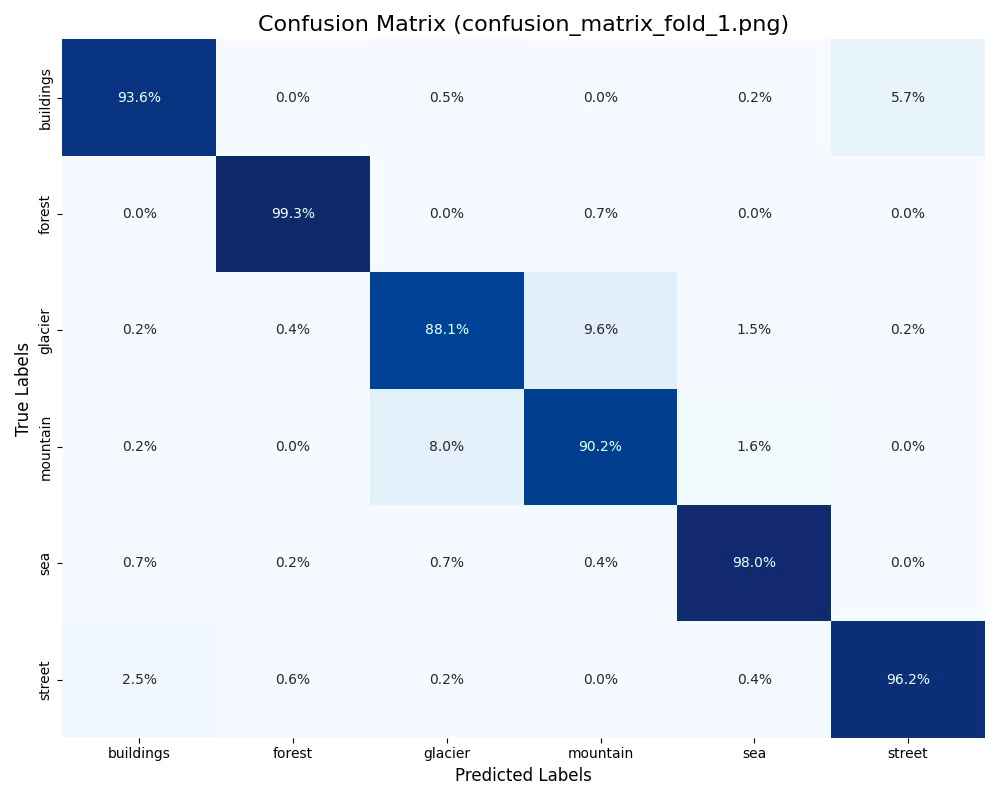
\includegraphics[width=\linewidth]{img/confusion_matrix_resnet50.png}
    \caption{Resnet50 Fold 1}
    \label{fig:conf_matrix_resnet}
\end{figure}

\begin{figure} 
    \centering
    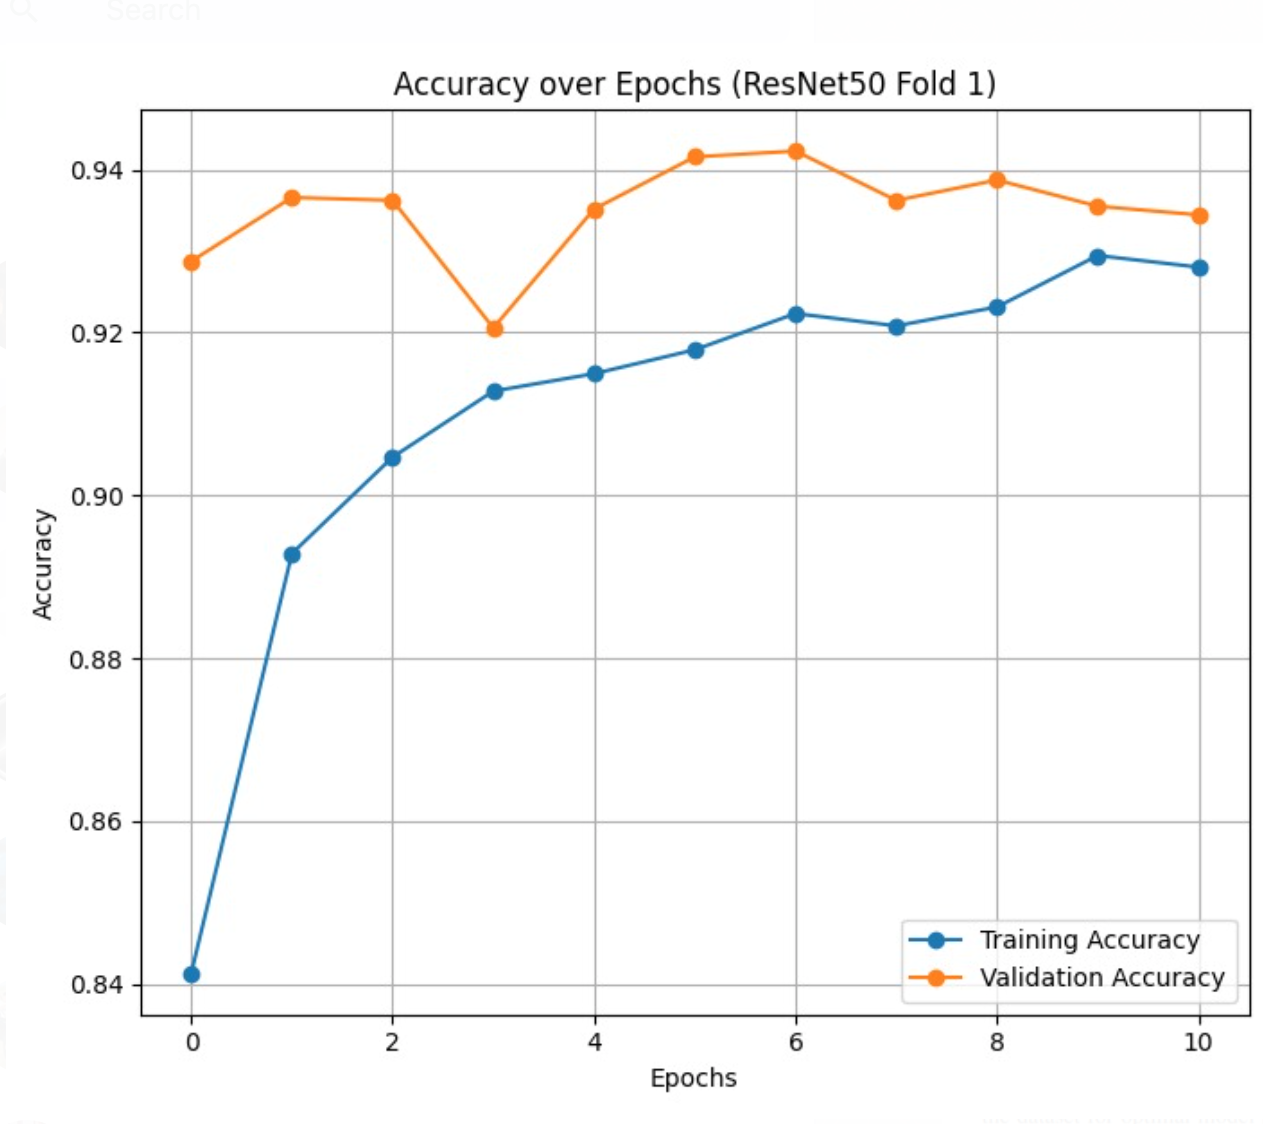
\includegraphics[width=\linewidth]{img/accuracyResnet50.png}
    \caption{Accuracy Over Epochs for Resnet50 Model Fold 1}
    \label{fig:accResnet}
\end{figure}

\begin{figure} 
    \centering
    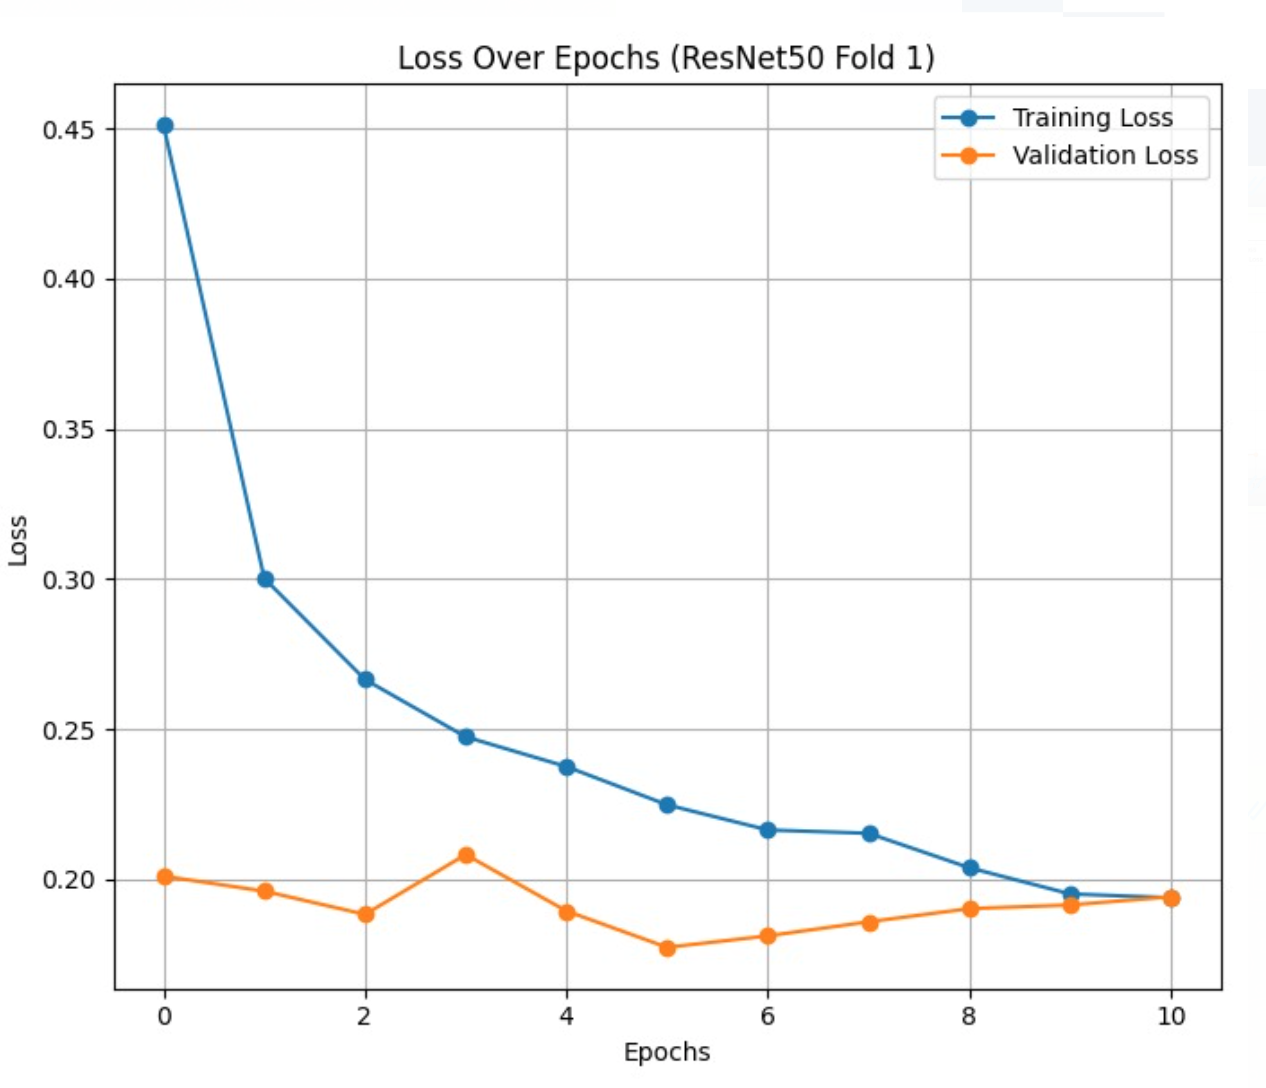
\includegraphics[width=\linewidth]{img/lossResnet50.png}
    \caption{Loss Over Epochs for Resnet50 Model Fold 1}
    \label{fig:lossResnet}
\end{figure}

The results indicate that the ResNet50 model consistently performed well across all folds, with minimal variance in metrics. The high Macro Average F1 Score and \ac{MCC} highlight the model's balanced performance across all classes.

\section{Results Comparison}
\label{sec:results}
% In order to test the best models in practice, some predictions were plotted using the best \ac{CNN} Layer Model, and the results are very positive in terms of classification when comparing the predicted and the expected class (Fig. \ref{fig:classesVis}). The model, out of 36 image prediction examples, got 6 wrong forecasts, which represent an accuracy of around 83\%.

% \begin{figure} [ht]
%     \centering
%     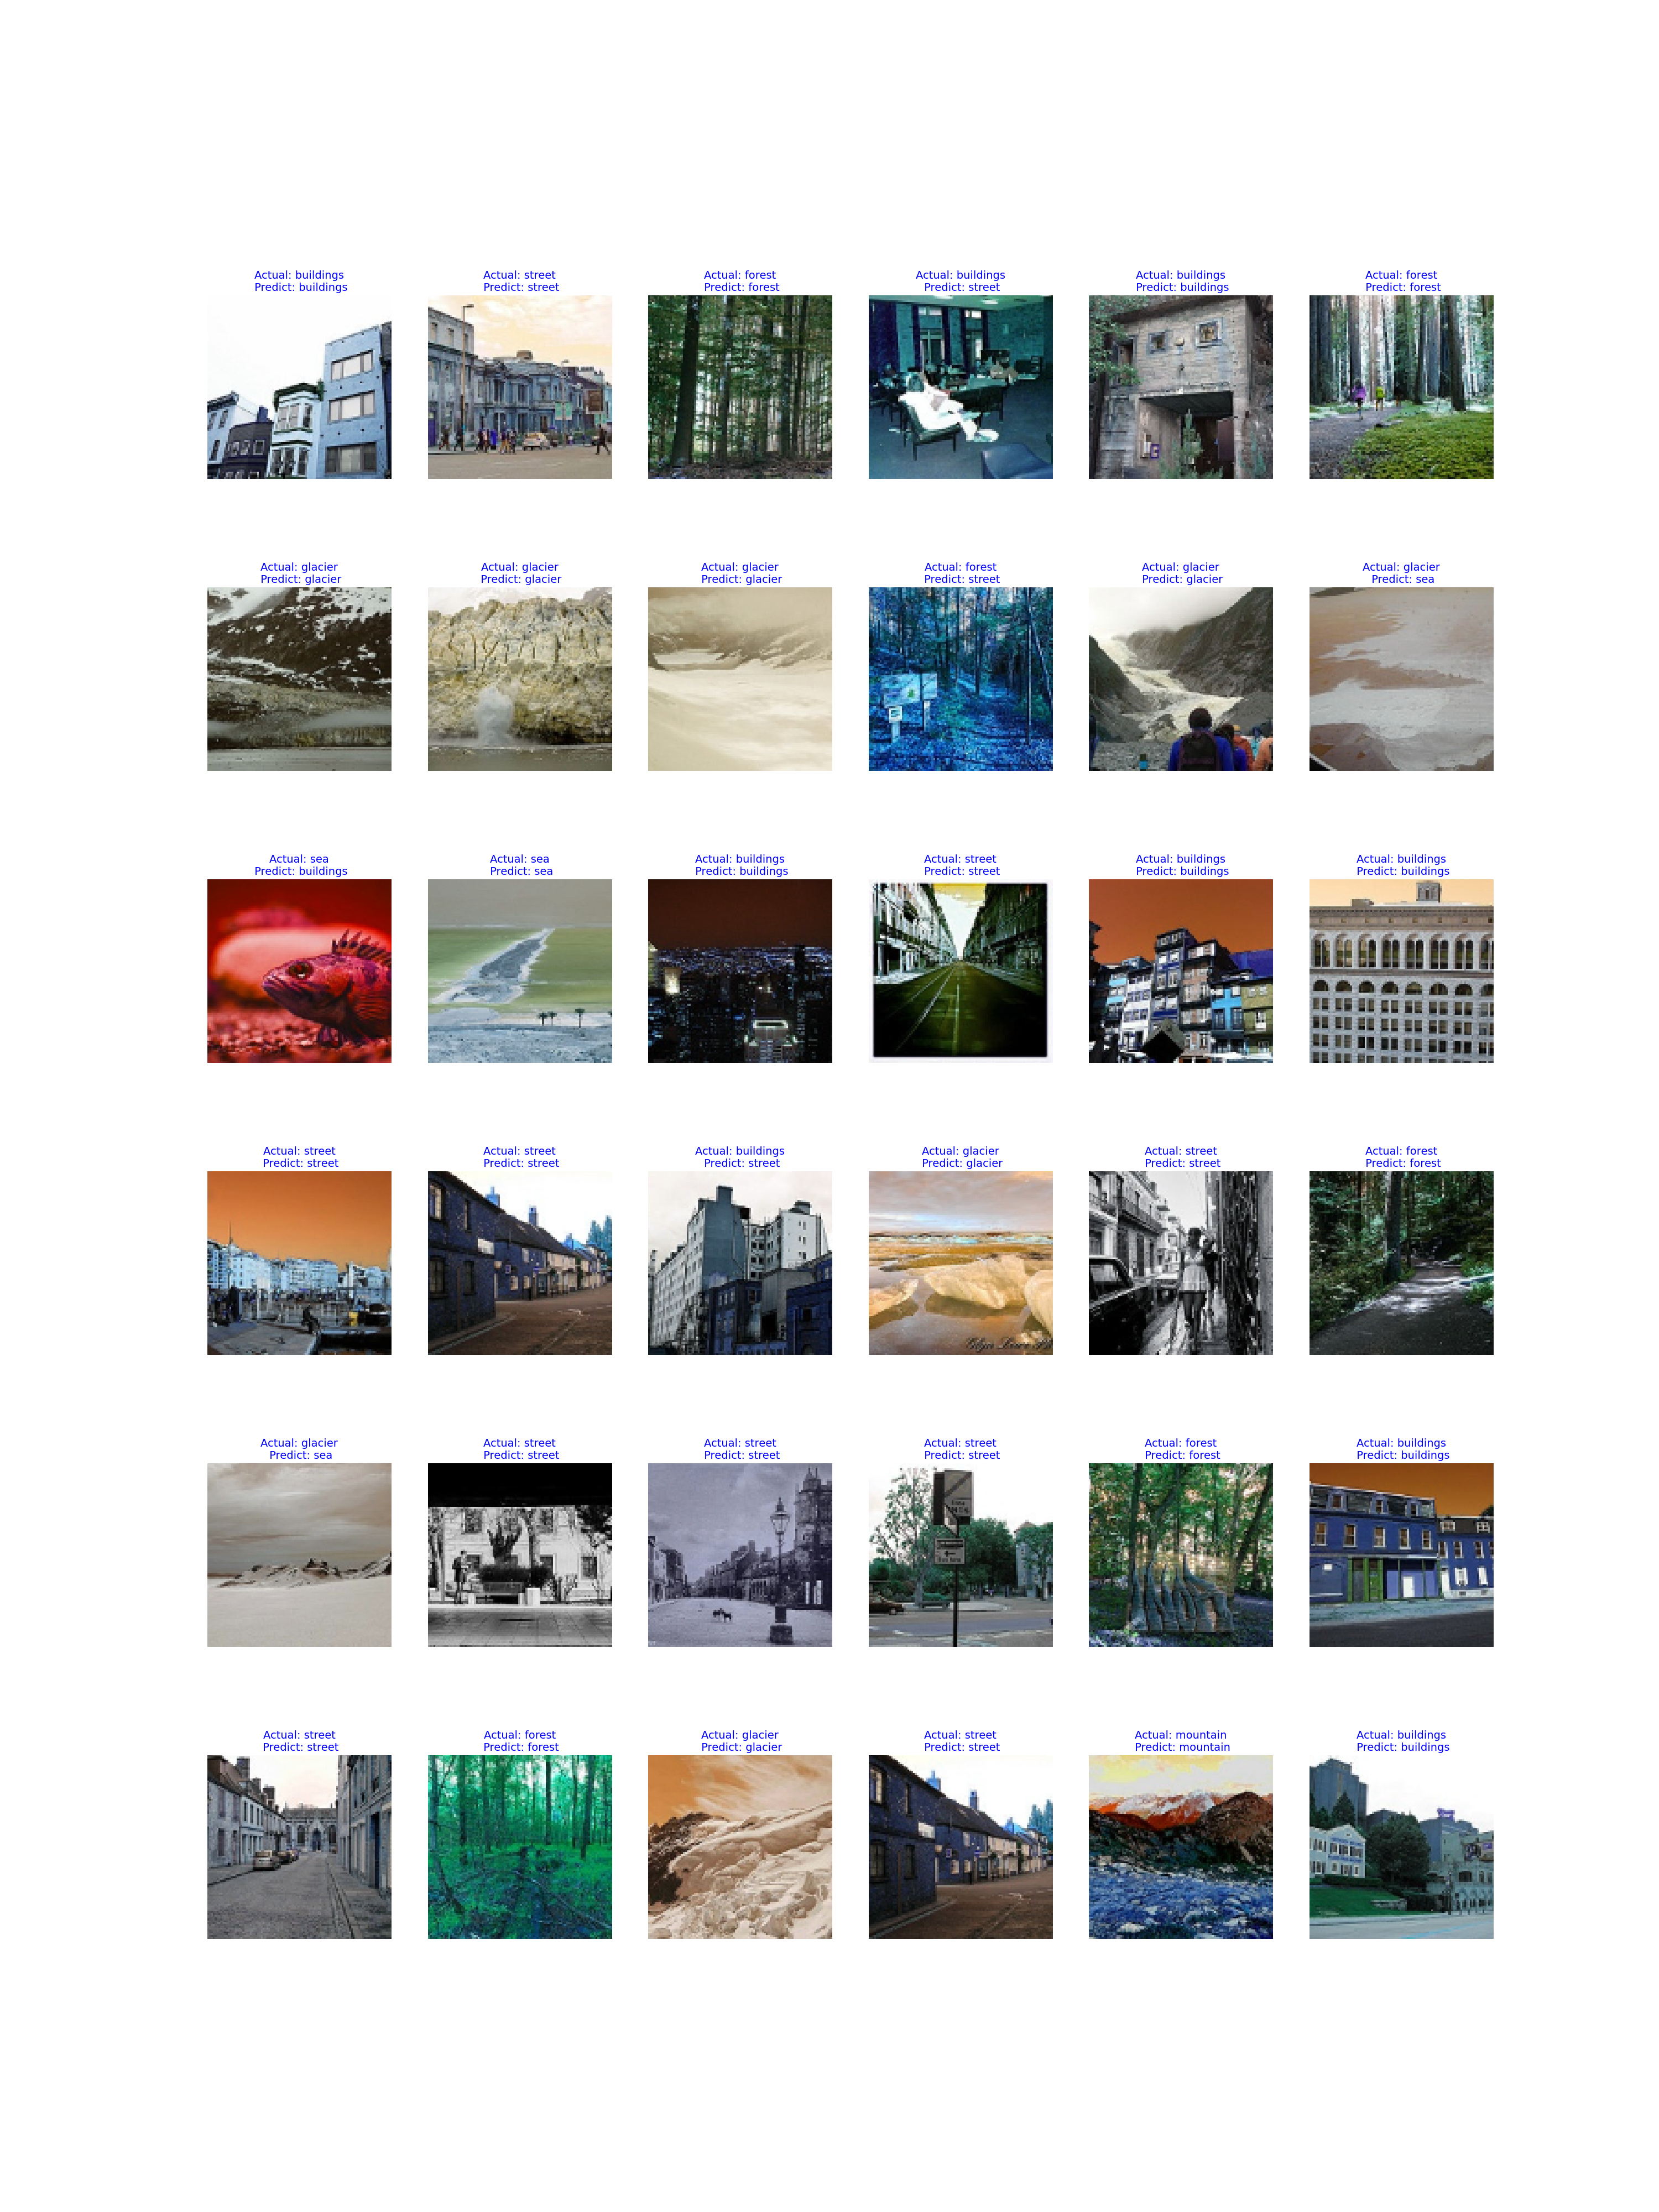
\includegraphics[width=\linewidth]{img/imagePredictionClass.png}
%     \caption{Image Prediction For the Best CNN 3 ConvLayer Model}
%     \label{fig:classesVis}
% \end{figure}

% MISSING RESULTS COMPARISON PROB A TABLE WITH ALL THE RESULTS AND A LIL EXPLANATION

\subsection{Model Performance Comparison}
In this section, the results are presented and compared to evaluate the performance of the different classification models used in this project. Table \ref{tab:comparison_models} summarizes the results and the key performance metrics across the used \ac{ML} models.

ResNet50 beats the other models, with an accuracy of 93.3\%, precision of 91.8\%, recall of 92.9\%, F1-Score of 92.9\%, and Matthews Correlation Coefficient (\ac{MCC}) of 0.929. This higher result demonstrates ResNet50's ability to handle complicated picture information and its robustness in classification challenges.

Following ResNet50, the Best \ac{CNN} model performs well with an accuracy of 82\%, precision of 83\%, recall of 83\%, F1-Score of 83\%, and \ac{MCC} of 0.80. In contrast, the Worst CNN has lower performance measures, including 65\% accuracy, 65\% precision, 65\% recall, 61\% F1-Score, and 0.59 \ac{MCC}. This gap demonstrates the impact of model architecture and training.

The Random Forest (\ac{RF}) model has a balanced performance, with around 60\% accuracy, precision, recall, and F1-Score, as well as an \ac{MCC} of 0.53. Meanwhile, the K-Nearest Neighbours (\ac{KNN}) model has the lowest performance across all metrics, with 41\% accuracy, 53\% precision, 40\% recall, 37\% F1-Score, and 0.30 \ac{MCC}.

Overall, the results show that \textbf{deep learning} models, particularly ResNet50, outperform classical machine learning approaches like \ac{KNN} and Random Forest in image landscape categorization. The large difference between the best and worst \ac{CNN} models highlights the relevance of model selection and training procedures in achieving optimal classification performance.

When comparing ResNet50 and the \ac{CNN} developed models, it is possible to conclude that Resnet50 performs better than the bespoke CNN model. Residual connections, a feature of ResNet50, help address the vanishing gradient issue and improve model training efficiency as network depth rises. Compared to a conventional CNN, this allows ResNet50 to extract more intricate and abstract features from the visual input. ResNet50's feature extraction skills are further enhanced by its well-optimized layer configuration and comprehensive validation on large-scale datasets. Together, these elements help ResNet50 achieve better results in the visual landscape classification challenge in terms of accuracy, precision, recall, and overall performance measures.

\begin{table}[ht]
    \centering  
    \begin{tabular}{|c|c|c|c|c|c|}
    \hline
    \textbf{Models} & \textbf{Accuracy} & \textbf{Precision} & \textbf{Recall} & \textbf{F1-Score} & \textbf{MCC} \\  \hline
    \ac{KNN} & 0.41 & 0.53 & 0.40 & 0.37 & 0.30 \\ \hline
    \ac{RF} & 0.61 & 0.60 & 0.60 & 0.60 & 0.53\\ \hline
    Worst \ac{CNN}               & 0.65            & 0.65                        & 0.65                     & 0.61                      & 0.59       \\ \hline
    Best \ac{CNN}               & 0.82            & 0.83                        & 0.83                & 0.83                        & 0.80 \\ \hline
    \textbf{Resnet50} & \textbf{0.933} & \textbf{0.918} & \textbf{0.929} & \textbf{0.929} & \textbf{0.929} \\ \hline
    \end{tabular}
    \caption{Performance Comparison of Models: KNN Vs Random Forest Vs Worst and Best CNN previously developed Vs Resnet50 }
    \label{tab:comparison_models}
\end{table}


\subsection{Comparison with Literature and Novel Contributions}
This study's findings show considerable advances in landscape image classification when compared to previous research. 

Our implementation of ResNet50 attained an accuracy of 93.3\%, which is comparable to the values published in other studies. For example, the GitHub repository that uses ResNet50 scored a test accuracy of 95.3\% \cite{githubpratim}. While slightly lower, our results are comparable to this benchmark, illustrating the durability of our approach in a multi-class classification environment. The small difference in accuracy could be ascribed to differences in experimental setups, such as data splits or augmentation procedures.

In contrast to Luo et al.'s study, which compared multiple machine learning models such as Random Forest, SVM, ANN, and CNNs \cite{luo2019}, our findings show that deep learning models such as ResNet50 outperform standard machine learning approaches. For example, our Random Forest implementation achieved just 61\% accuracy, which is much lower than ResNet50's 93.3\%, highlighting the limitations of traditional approaches in dealing with complicated image data.

Our findings are consistent with those of S. Thirumaladevi et al. \cite{Thirumaladevi} and Wenmei Li et al. \cite{Li}, who emphasized the benefits of transfer learning for scene classification tasks. Both research found that adjusting pre-trained models such as ResNet50 to fresh datasets greatly improves classification performance. Our findings further confirm this strategy by proving its suitability for the Intel Image Classification dataset.

While previous research, such as that by Luo et al. \cite{luo2019} and Zeng et al. \cite{zeng}, provides broad overviews of scene classification algorithms, our work focuses on the comparative performance of specific models, providing practical insights into their strengths and limits. The significant disparity between ResNet50 and other models, such as KNN and Random Forest, emphasizes the importance of using deep learning architectures for complicated picture classification.

\section{Conclusion}
\label{sec:concl}
This project, developed for the course ''Foundations of Machine Learning'' - ''Fundamentos de Aprendizagem Automática'' in Portuguese - explored the application of machine learning models for image landscape classification. Utilizing a diverse Kaggle dataset with six categories, namely buildings, forests, glaciers, mountains, seas, and streets. The study aimed to identify and understand, from the given data, the most effective and suitable classification model, as well as to assess how model architecture influences classification performance.

It was shown that deep learning techniques perform better than conventional machine learning techniques by extensive data preprocessing and testing with several models, such as K-Nearest Neighbours (\ac{KNN}), Random Forest (\ac{RF}), and multiple Convolutional Neural Networks (CNNs). ResNet50, which used its sophisticated design and residual connections to precisely classify intricate visual features, notably earned the best performance.

The outcomes demonstrate how well deep learning models, in particular, ResNet50 perform complex picture classification tasks. This experiment emphasizes how crucial model selection and training techniques are to attaining peak performance. To further increase classification accuracy and model suitability for generalization, future research should investigate more deep learning architectures, better data augmentation methods, hyper parameter tuning and enlarge the dataset.



% MISSING CONCLUSION + Future work


\section{Acronyms}
\begin{acronym}
    \acro{ML}{Machine Learning}
    % \acro{LR}{Logistic Regression}
    % \acro{NN}{Neural Networks}
    \acro{CNN}{Convolutional Neural Network}
    % \acro{SVM}{Support Vector Machine}
    \acro{RF}{Random Forest}
    \acro{KNN}{k-Nearest Neighbors}
    % \acro{ROC}{Receiver Operating Characteristic Curve}
    % \acro{AUC}{Area Under the Curve}
    \acro{MCC}{Matthews Correlation Coefficient}
    % \acro{MSE}{Mean Squared Error}
\end{acronym}

\begin{thebibliography}{00}

\bibitem{kri2017} Krizhevsky, A., Sutskever, I., and Hinton, G. E., “ImageNet Classification with Deep Convolutional Neural Networks,” Communications of the ACM, vol. 60, no. 6, pp. 84–90, June 2017. DOI: 10.1145/3065386

\bibitem{kaggleDataset} Puneet, “Intel Image Classification Dataset,” Kaggle, [Online]. Available: \url{https://www.kaggle.com/datasets/puneet6060/intel-image-classification?resource=download}. [Accessed: Dec. 14, 2024]

\bibitem{luo2019} Luo, Y., Li, P., Fu, S., \& Shi, Y. (2019). Natural Scene Images Classification.
Department of Structural Engineering and Electrical Engineering, University of California, San Diego (UCSD)

\bibitem{githubpratim} M. Pratim, Intel Image Classification, GitHub repository, 2020. [Online]. Available: \url{https://github.com/manashpratim/Intel-image-Classification}. [Accessed: Dec. 15, 2024]

\bibitem{zeng} Z. Delu, M. Liao, M. Tavakolian, Y. Guo, B. Zhou, D. Hu, M. Pietikainen, and L. Liu, "Deep Learning for Scene Classification: A Survey," IEEE Transactions on Pattern Analysis and Machine Intelligence, vol. 41, no. 9, pp. 2130-2147, Sept. 2019. doi: 10.1109/TPAMI.2018.2880899

\bibitem{Thirumaladevi} S. Thirumaladevi, K. Veera Swamy, and M. Sailaja, "Remote sensing image scene classification by transfer learning to augment the accuracy," J. of Electr. and Electron. Eng., vol. 14, no. 5, pp. 82-89, 2020

\bibitem{Li} W. Li, Z. Wang, Y. Wang, J. Wu, J. Wang, Y. Jia, and G. Gui, "Classification of high-spatial-resolution remote sensing scenes method using transfer learning and deep convolutional neural network," IEEE Trans. Geosci. Remote Sens., vol. 58, no. 6, pp. 4210-4221, Jun. 2020, doi: 10.1109/TGRS.2019.2948154

\bibitem{normalization} J. Brownlee, "A Gentle Introduction to Normality Transformation for Machine Learning," Machine Learning Mastery, 2019. [Online]. Available: \url{https://machinelearningmastery.com/a-gentle-introduction-to-normality-transformation-for-machine-learning/}. [Accessed: Dec. 20, 2024]

\bibitem{ImageDataGenerator}TensorFlow, "tf.keras.preprocessing.image.ImageDataGenerator," TensorFlow, 2024. [Online]. Available: \url{https://www.tensorflow.org/api\_docs/python/tf/keras/preprocessing/ image/ImageDataGenerator.} [Accessed: Dec. 20, 2024]

\bibitem{encoding}
I. Rahadhian, "One-Hot Encoding: What and Why," Medium, 10-Dec-2020. [Online]. Available: \url{https://medium.com/@irvan.rahadhian/one-hot-encoding-what-and-why-f22d11a7602a}. [Accessed: Dec. 20, 2024]

\bibitem{deeplizard} Deeplizard, "Deep learning with convolutional neural networks," [Online]. Available: \url{https://deeplizard.com/learn/video/YRhxdVk_sIs}. [Accessed: Nov. 18, 2024]

\bibitem{softmaxactivation} Pinecone, "Softmax Activation: A Beginner's Guide," Pinecone.io, [Online]. Available: \url{https://www.pinecone.io/learn/softmax-activation/}. [Accessed: Dec. 30, 2024]

\bibitem{relumax} Es-sabery, Fatima \& Hair, Abdellatif \& Qadir, Junaid \& Sainz de Abajo, Beatriz \& Garcia-Zapirain, Begona \& De la Torre Díez, Isabel. (2021). Sentence-Level Classification Using Parallel Fuzzy Deep Learning Classifier. IEEE Access. PP. 1-1. 10.1109/ACCESS.2021.3053917

\bibitem{adam} Keras, "Adam Optimizer," Keras.io, [Online]. Available: \url{https://keras.io/api/optimizers/adam/} [Accessed: Dec. 30, 2024]

\bibitem{crossentropy} Pareto.ai, "Understanding Cross-Entropy Loss Function," Pareto.ai, [Online]. Available: \url{https://pareto.ai/blog/cross-entropy-loss-function\#:~:text=Categorical\%20cross\%2Dentropy\%20loss\%20is,and\%20the\%20actual\%20categorical\%20labels} [Accessed: Dec. 30, 2024]

\bibitem{earlyStopping} Cyborg Codes, "What is Early Stopping in Deep Learning?," Medium, [Online]. Available: \url{https://cyborgcodes.medium.com/what-is-early-stopping-in-deep-learning-eeb1e710a3cf}. [Accessed: Dec. 30, 2024]

\bibitem{confmatrix} GeeksforGeeks, "Confusion Matrix in Machine Learning," GeeksforGeeks, [Online]. Available: \url{https://www.geeksforgeeks.org/confusion-matrix-machine-learning/}. [Accessed: Dec. 30, 2024]

\bibitem{classreport} Scikit-learn, "sklearn.metrics.classification\_report — scikit-learn 1.5.0 documentation," 2024. [Online]. Available: \url{https://scikit-learn.org/1.5/modules/generated/sklearn.metrics.classification_report.html}. [Accessed: Dec. 30, 2024].

\bibitem{b3} A. Géron, *Hands-On Machine Learning with Scikit-Learn, Keras, and TensorFlow*. O'Reilly Media, 2019.

\bibitem{logloss} Analytics Vidhya, "Log Loss vs. Mean Squared Error: Choosing the Right Metric for Classification" [Online]. Available: \url{https://tinyurl.com/ytrx5fyx}. [Accessed: Nov. 18, 2024].

\bibitem{loglosss} C. Bathula, "Mastering Multi-Class Log Loss: A Comprehensive Guide to Boost Your Machine Learning Skills," Medium, Oct. 23, 2023. [Online]. Available: https://medium.com/@chandu.bathula16/mastering-multi-class-log-loss-a-comprehensive-guide-to-boost-your-machine-learning-skills-fbbc74f63c7. [Accessed: Nov. 16, 2024].

\bibitem{imagenet} J. Deng, W. Dong, R. Socher, L.-J. Li, K. Li, and L. Fei-Fei, "ImageNet: A large-scale hierarchical image database," 2009 IEEE Conference on Computer Vision and Pattern Recognition, Miami, FL, USA, 2009, pp. 248–255, doi: 10.1109/CVPR.2009.5206848. 

\end{thebibliography}

\vspace{12pt}
\color{red}


\end{document}
